% Configuration for Phase Method
\subsection{Fixed Frequency Value}
\label{subsec:04_fixedFrequencyVal}

In order to decide on a fixed frequency for the phase method,
resulting errors of different frequency were evaluated.
For this, all measurements in \cref{subsec:04_labMeasurements}
of the robot 26 at the center point are utilized.
As the \ac{RMSE} in \cref{fig:04_diffFc} shows, for frequencies smaller
than 2600\si{\hertz} the errors are much higher.
With a frequency of 2024.12\si{\hertz}, error is largest.
The fixed frequency is set to 2627,1\si{\hertz} according
to the smallest \ac{RMSE}.
% -------------------------------------------------------------
\begin{figure}[ht]
	\centering
		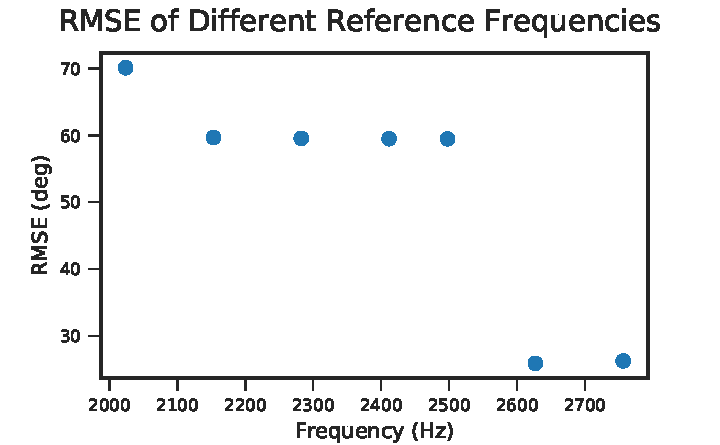
\includegraphics[]{figures/evaluation/phase_fc_rmse}
	\caption{Result of all measurements for Nao 26 to compare different
	fixed frequency values.}
	\label{fig:04_diffFc}
\end{figure}
% -------------------------------------------------------------
\subsection{Frame Number}
\label{subsec:04_frameNumber}

Not only does the frequency play a role for the phase method,
but also the frame chosen.
To evaluate if the result changes over time, the frame to
utilize is shifted by half the frame size for all measurements
of \cref{subsec:04_labMeasurements} for the robot at the center
point.
% [ 29.08029745  58.1426789   65.27548831  67.91984464  76.82890558
%   97.33976251  96.63736674 100.2203543  105.14752253  61.28179302
%   60.0017076   50.60063622  53.80158271  49.0830362   62.64453085]
In \cref{fig:04_phaseOverTime} we see, that the first channel frames
with zero shift gives the best result with a \ac{RMSE} of 29,1\si{\degree}.
This again shows us, that the signal start detection plays a
large role for the correct result.
% -------------------------------------------------------------
\begin{figure}[ht]
	\centering
		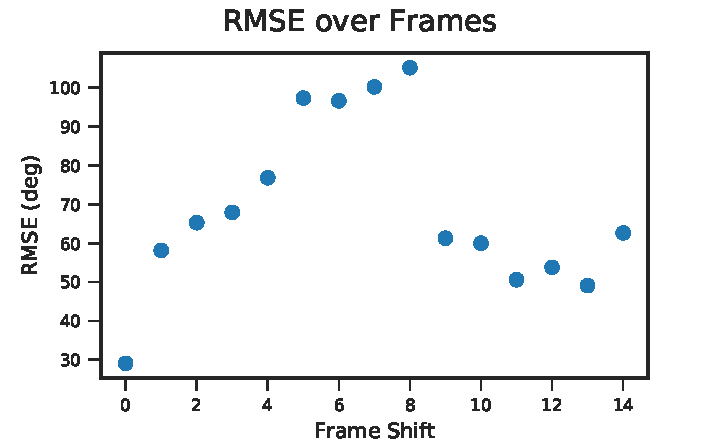
\includegraphics[]{figures/evaluation/phase_over_time}
	\caption{}
	\label{fig:04_phaseOverTime}
\end{figure}
% -------------------------------------------------------------